%
% 公立はこだて未来大学卒業研究中間報告書[全コース対応版]
%
%         ファイル名:"sample.tex"
%
\documentclass[11pt]{ujarticle}
\usepackage{subfig}
\usepackage{funinfosys}
\usepackage{url}
\usepackage[dvipdfmx]{graphicx}
\usepackage{url}

\author{% 
1020259 中村碧\\指導教員 : 松原克弥
}
\course{Intelligent Systems Course}

\title{クラウド-ロボット間でROSノードが移行できるアーキテクチャ中立なROSランタイムの実現に向けたmROS2-POSIXの評価}
\etitle{}
\eauthor{Aoi Nakamura}
\abstract{
ロボットソフトウェア開発において、ROSの利用が増加している.
クラウド連携を用いた分散ロボットシステムの構築が主流だが、ノード配置の柔軟性が課題となっている.
特に、クラウドとロボットのCPUアーキテクチャの違いから、動的なノード再配置が難しい.
先行研究での動的配置機構はオーバーヘッドの増加が問題とされ、mROS 2-POSIXを用いたアプローチも提案されているが、評価は小規模アプリケーションに限定されている.
\\本研究では、mROS 2-POSIXを用いてROS 2の性能を評価.通信性能やメモリサイズを基に、動的配置機構の可能性を検証する.
}
\keywords{ロボティクス,mROS2-POSIX}
\eabstract{In robot software development, the use of ROS is on the rise. While building distributed robot systems through cloud integration is popular, the flexibility in node placement remains a challenge. Specifically, the disparity in CPU architectures between the cloud and robots complicates dynamic node reallocation. Previous studies on dynamic placement mechanisms have reported increased overhead, and although approaches using mROS 2-POSIX have been proposed, evaluations have been limited to small-scale applications.
\\ In this research, we evaluate the performance of ROS 2 using mROS 2-POSIX. Based on communication performance and memory size, we explore the potential of dynamic placement mechanisms.}
\ekeywords{Roboethics, mROS2-POSIX}
\begin{document}
\maketitle
%\vspace*{-.5cm}

\section{背景と目的}
\label{sec:introduction}
さまざまな産業向けやエンターテイメント関連のロボットシステム,自動車の自動運転技術やIoTシステムの構築においても,これらのソフトウェア開発をサポートするフレームワークとしてRobot Operating System(以下,ROS)の普及が増加している[1].ROSのプログラミングモデルは,システムの各機能を独立したプログラムモジュール(ノード)として設計することにより,汎用性と再利用性を向上させて,各機能モジュール間のデータ交換を規定することで,効率的かつ柔軟なシステム構築を可能にしている.たとえば,カメラを操作して周囲の環境を撮影するノード,画像からオブジェクトを識別するノード,オブジェクトのデータを基に動作制御を実行するノードを連携させることで,自動運転車の基本機能の一部を容易に実装できる.
\\ ROSのプログラミングモデルは,ロボット/IoTとクラウドが協力する分散型システムにおいても有効である.ロボットシステムのソフトウェア処理は,外界の情報を取得する「センサー」取得した情報を処理する「知能・制御系」実際に動作するモーターなどの「動力系」の3要素に分類できる[2].クラウドロボティクス[3]において,主に知能・制御系のノードを高い計算能力を持つクラウドに優先して配置することで,高度な知能・制御処理の実現を促進しできる.
さらに,必要な情報をクラウドに集約・保存することで,複数のロボット間での情報共有と利用を容易にする.
一方で,現行のROS実装においては,各ノードの配置をシステム起動時に設定する必要があり,先述のクラウドロボティクスのクラウドとロボット間の最適なノード配置を事前に設計する必要がある.しかし,実際の環境で動作するロボットは,ネットワークの状況やバッテリー残量の変動など,システム運用前に予測することが困難な状況変化に対応する必要があり,設定したクラウドとロボット間のノード配置が最適でなくなる可能性がある.このような状況変化に対する対応として,ノードを動的に再配置するマイグレーション機能の実現が求められているが,多くの場合でクラウドとロボット間のCPUアーキテクチャが異なり,実行中のノードをシステム運用中にマイグレーションすることは技術的に困難である.
\\ 菅らは,WebAssembly(以下,Wasm)を用いることで,クラウドとロボット間での実行状態を含む稼働中ノードの動的なマイグレーションする手法を実現した[4].
課題として,ROS 2をWasm化したことでオーバーヘッドが増大し,マイグレーション後,ノードの実行時間が大幅に増えてしまう問題が残った.
柿本ら[5]は,組込みデバイス向けROS 2ランタイム実装であるmROS 2-POSIXを採用し,ROSランタイムのWasm化にともなうオーバヘッド増加に対処した.
しかし,採用されたmROS 2-POSIXはごく小規模なアプリケーション上でしか評価実験は行われておらず[6],動的配置機構を実装するソフトウェア基盤としてmROS2 POSIXを採用する上で,アプリケーションの規模を増加させた評価実験は必要不可欠である.
\\ 本研究では,クラウドとロボット間での実行状態を含む稼働中ノードの動的マイグレーションの実現に向けたmROS 2-POSIXの性能評価を行い,mROS 2がROS 2と比べて動的配置機構の実現のソフトウェア基盤としてどの点で優位性があるのか明らかにすることを目指す.
%目的



\section{mROS2-POSIX}
mROS 2は,ROS 2ノードの軽量実行環境である.
mROS 2は,中規模の組込みデバイス上で事項されるプログラムに汎用デバイス上のROS 2ノードと自律的に通信する機能を提供している.
このソフトウェア基盤によって,分散型のロボットシステムへの組込み技術の導入できる.
組込みデバイスは計算資源が限定的であるが,リアルタイム性の向上および消費電力が削減をできる.
そして,mROS 2がPOSIX[7]に対応したのがmROS 2-POSIXである.
\\ 図1(a)は,mROS 2-POSIXのソフトウェア構成を示す.mROS 2-POSIXアプリケーション層は,ユーザが実装するROS 2ノードに相当する.
\begin{figure}[t]
	\centering
	\begin{minipage}{.5\textwidth}
		\centering
		\subfloat[mROS 2-POSIXの内部構成]{
			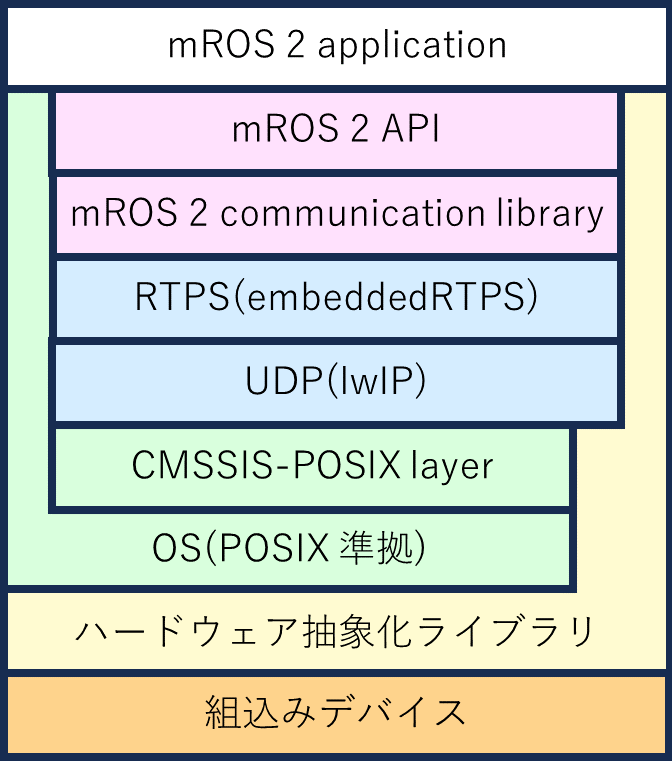
\includegraphics[width=0.45\textwidth]{./src/fig1_mros2posix_a.png}\label{fig:subfig_a}
		}
		\hfill
		\subfloat[mROS 2の内部構成]{
			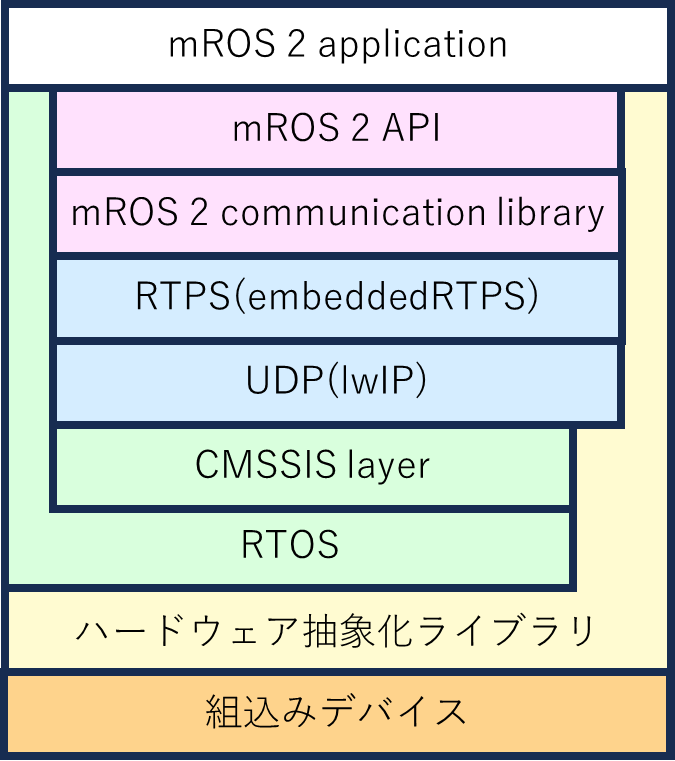
\includegraphics[width=0.45\textwidth]{./src/fig1_mros2_b.png}\label{fig:subfig_b}
		}
	\end{minipage}
	\caption{mROS 2-POSIXとmROS 2のソフトウェア構成}
	
\end{figure}
mROS 2-POSIX API層および通信ライブラリ層は,ROS 2のtopicに相当するAPIおよび通信機能を提供する階層である.
本階層は,ROS 2のネイティブなクライアント通信ライブラリであるrclcppと互換性を保つように設計している.
mROS 2通信ライブラリでは,rclcppのうちpub/sub通信の基本的な機能のみ実装されている.
利用可能な機能は制限されているものの,組込み技術を導入するROS 2開発者は,汎用OS向けのプログラミングスタイルを踏襲しながらC++によってmROS 2のアプリケーションを実装できる.
\\ Real Time Publish-Subscribe(以下,RTPS)プロトコルスタックにはUDPでパブリッシャとサブスクライバC++実装のembeddedRTPS[8]が採用されている.
また,RTPSにおけるSPDPおよびSEDPが実装されているため,通信の自立性が実現できる.
UDPについては組込み向けのC実装であるlwIPが採用されている.
また,これらの階層はCMSIS-POSIX APIに依存している.
通信層のembeddedRTPSおよびlwIPはCMSAIS-POSIXに依存しており,図1(b)に示すmROS 2のCMSIS-RTOSを互換した層になっている.
最下層にはハードウェアを抽象化したライブラリがある.
\\ mROS 2-POSIXの実行方式は,mROS 2が対応しているリアルタイムOSとの相違がある.
リアルタイムOSでは,組込みマイコンを実行資源の管理対象として,タスク単位でアプリケーションが実行される.
POSIXにおいてはタスクに相当する概念はプロセスであり,そこから生成されるスレッドを実行単位として処理が進行している.
\\ したがって,mROS2-POSIXは図2に示す実行方式を採用している.
\begin{figure}[t]
	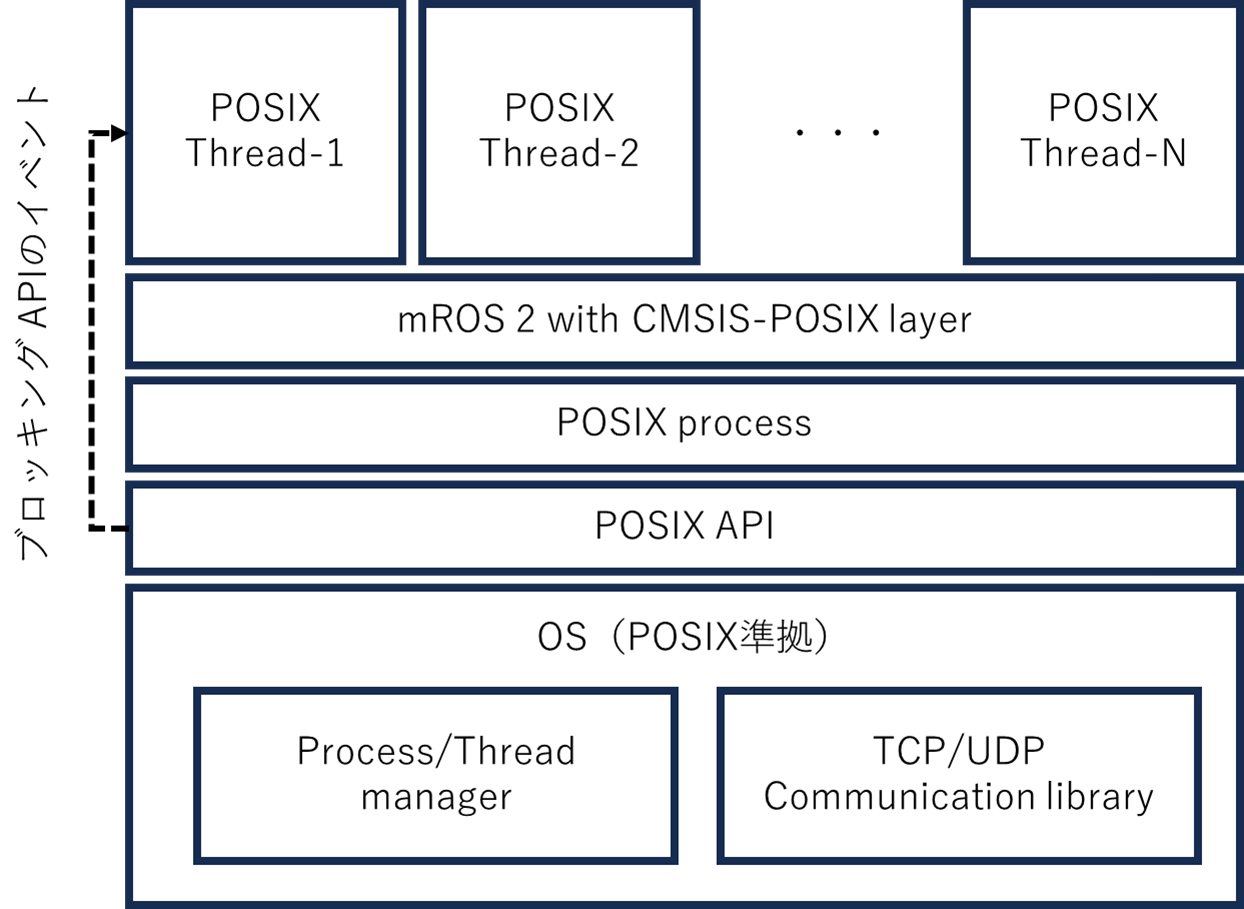
\includegraphics[width=0.7\linewidth]{./src/fig2_execution_structure.png}
	\caption{mROS 2-POSIXの実行方式}
  \label{fig:arch}
\end{figure}
mROS 2-POSIXの実行単位であるノードはPOSIXのスレッドに対応付けらており,mROS 2の通信ライブラリ機能を担う実行資源はPOSIXのプロセスとして捉え,これを管理対象としている.
組込みマイコンでの通信処理におけるイベント割込みについては,POSIX準拠OSにおけるブロッキングAPIの発行に相当させて処理されている.
\\ mROS 2とmROS 2-POSIXの機能構造の対応として,タスク管理機能は,スレッドの生成や開始などのPOSIX資源の管理機能に対応付けれている.
メッセージキューおよびミューテックスによるスレッドの同期・通信および排他制御は,POSIXではPthreadによって対応している.
メモリ管理機能はAlloc/Freeで,時間管理はOS時刻管理機能で対応している.
lwIPにおけるUDPパケット処理は,POSIXにおけるOS資源の操作に関する機能で実現されている.
\\ 先行研究である菅ら[4]と柿本ら[5]は動的配置機構を実装する環境の想定として,クラウドのCPUアーキテクチャはx64 PC,組込みデバイスはarm64 RPi4上のUbuntuで動作することを想定している.
mROS 2-POSIXはmROS 2とは違い,POSIXに準拠したUbuntuを動作させることができる.
本研究では,mROS 2-POSIXとROS 2を比較評価し,その性能が動的配置機構の実現に向けたソフトウェア基盤として適切であるか評価する. 

\section{評価方針}
mROS 2-POSIXを評価するにあったって,mROS2と同様のアプリケーションをROS 2に実装し,比較評価する.
mROS 2は,ROS2に同様のアプリケーションを実装した場合でも期待される動作をすることができる.
評価に使用するアプリケーションはSphero SPRK+とWii Fit Boardを用いたロボット制御アプリケーションである.
アプリケーションは,Wii Fit Boardはユーザの体重移動を検知し,Sphero SPRK+を前後左右に動かすことで,ユーザの体重移動に追従するように動作する.
図3にアプリケーションの構造を示す.
\begin{figure}[t]
	\centering
	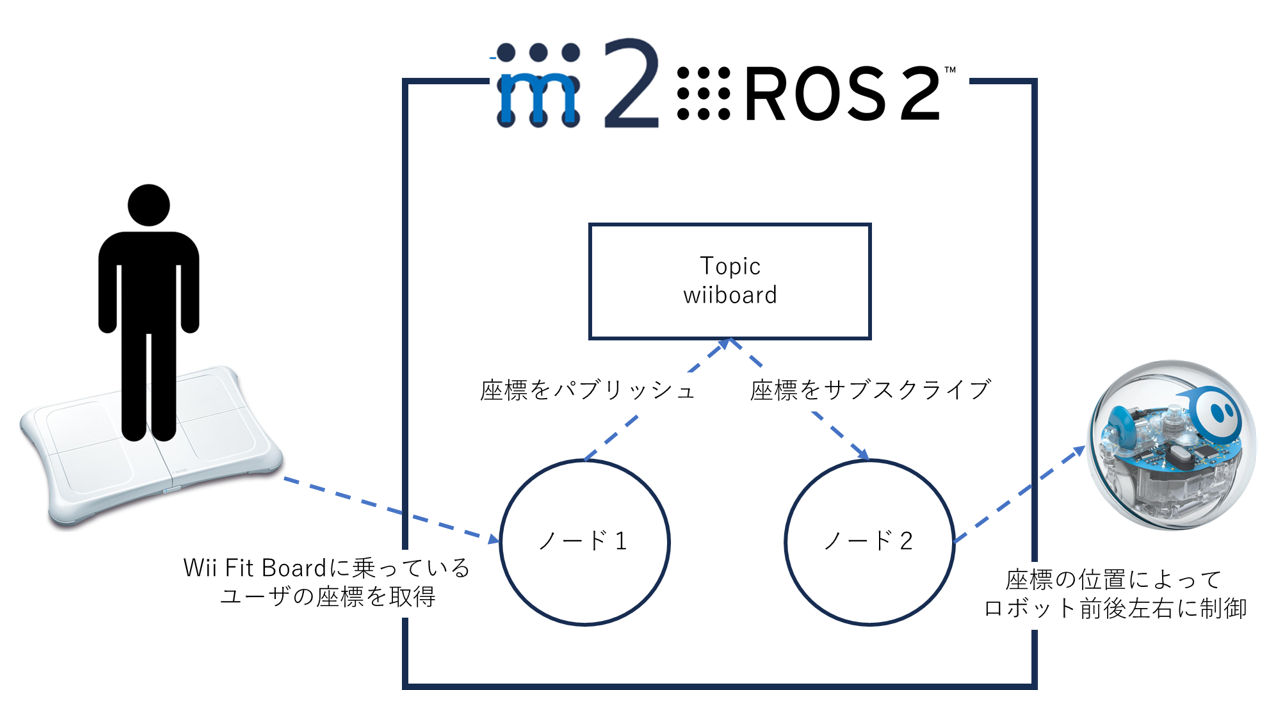
\includegraphics[width=0.75\linewidth]{./src/fig3_application_structure.png}
	\caption{実装するアプリケーション}
  \label{fig:arch}
\end{figure}
mROS 2-POSIXは,ごく小規模なアプリケーション上で評価されており[],図3のようなハードウェアを通して利用されるアプリケーションの評価は行われていない.
したがって,本研究では規模を大きくしたアプリケーションを実装し,mROS 2-POSIXの評価を行う.
Wii Fit Boardに乗っているユーザの座標をパブリッシュするノードであると,Wii Fit BOardの座標があるトピックにサブスクライブし,受け取った値をもとにSphero SPRK+を動作させるノードの2つにわけられる.
評価項目としては,mROS 2-POSIXがROS 2と比べてどの点で優位性があるのかを明らかにするため,以下の項目を設定した.
\begin{itemize}
	\item 通信性能の評価
	\item メモリサイズの評価
\end{itemize}
 通信性能の評価については,1回の通信をWii Fit Boardの値をサブスクライブするまでとし,それを100回行い,その平均と最大値と最小値と標準偏差を取ることで性能比較を行う.
\\メモリサイズの評価については,アプリケーションのバイナリをsizeコマンドで計測しそれぞれtext,data,bssのサイズを比較する.

\section{評価アプリケーションの実装}
% Wii Fit BoardとSphero SPRK+を用いたロボット制御アプリケーションは,Wii Fit Boardはユーザの体重移動を検知し,Sphero SPRK+を前後左右に動かすことで,ユーザの体重移動に追従するように動作する.
% 評価アプリケーションの実装として,mROS 2-POSIXとROS 2の両方で同じ機能を持つノードを作成する必要がある.
ROS 2のアプリケーションは,Wii Fit Boardの値を取得するOSSをROS 2ノード化したものと,Sphero SPRK+を動作させることができるライブラリを提供しているOSSをROS 2ノード化して通信させている.
mROS 2-POSIXのアプリケーションの実装はROS 2のアプリケーションの機能と同じものを実装する必要があるため,同様のものを作成する.
ROS 2で動作するノードのソースコードはそのまま移植することはできないため,ROS 2のrclcppではなくmROS 2-POSIX固有のAPIを使用して作成する必要がある.
また,Sphero SPRK+を動作させるライブラリはPythonでコーディングされているため,C++のみしか対応していないmROS 2-POSIXではそのまま使用できないので,C++のライブラリに書き換える必要がある.
\section{進捗と計画}
現在の進捗状況として,アプリケーションはROS 2で動作するノードの作成が完了した.
mROS 2-POSIX対応は未実現である.
mROS 2-POSIXでは,Wii Fit Boardの値をパブリッシュするノードは移植することができた.
Sphero SPRK+のノードの移植は,ライブラリがPythonで書かれているため,C++に書き換える必要がある.

\section{結言}
本研究では,クラウドとロボット間での実行状態を含む稼働中ノードの動的マイグレーションの実現に向けたmROS 2-Posixの評価を行い,mROS 2がROS 2と比べて動的配置機構の実現のソフトウェア基盤としてどの点で優位性があるのか明らかにすることを目指す.
\\ 動的配置機構の手法をROS 2環境で実現した菅ら[4]はオーバーヘッドの増加が課題であるとしている.
柿本ら[5]は,mROS 2-POSIXを用いたアプローチを提案している.
しかし,mROS 2-POSIXを評価している研究[6]ではROS 2とmROS 2-POSIXの通信性能とメモリサイズを評価しているが,ごく小規模なアプリケーションで評価を行っている.
そのため,本研究では,mROS 2-POSIXを用いてROS 2の性能を評価.通信性能やメモリサイズを基に,動的配置機構の可能性を検証する.
\section{知能システムコースにおける本研究の位置づけ}
本研究は,ROS 2の組込み向けデバイスでの実行環境であるmROS 2-POSIXの評価を行うことで,クラウドとロボット間での実行状態を含む稼働中ノードの動的マイグレーションの実現に向けたソフトウェア基盤としての優位性を明らかにすることを目指している.
その過程で,mROS 2-POSIXで動作するロボット制御アプリケーションの実装を行い,アプリケーションの動作を評価することで,動的配置機構を実装するソフトウェア基盤として適切であるか評価する.
そのため,知能システムコースのカリキュラムポリシーに記載のある「実世界への実装に関する具体的な課題に取り組み,その結果の評価を通じて,新しい方法論や学問領域を切り拓く能力を育む」に該当する.


\begin{thebibliography}{99}
	\bibitem{ros}
	ROSWiki:ROS/Introduction, url{http://wiki.ros.org/ROS/Introduction.}
	\bibitem{robotkenkyuukai}
	ロボット政策研究会: ロボット政策研究会 報告書 ~RT革命が日本を飛躍させる~,\url{https://warp.da.ndl.go.jp/info:ndljp/pid/286890/www.meti.go.jp/press/20060516002/robot-houkokusho-set.pdf (2006).}
	\bibitem{cloudrobotics}
	Kehoe et al. explored cloud-based robot grasping utilizing the Google object recognition engine, presenting their findings in the 2013 IEEE International Conference on Robotics and Automation, pages 4263-4270.
	\bibitem{kan}
	菅文人,松原克弥: クラウドロボティクスにおける異種デバイス間タスクマイグレーション機構の検討,研究報告組込みシステム(EMB),Vol. 2022, No. 36, pp. 1-7(2022).
	\bibitem{kakimoto}
	柿本翔大,松原克弥:クラウド連携を対象としたアーキテクチャ中立なROSランタイムの実現,情報処理学会研究報告, Vol. 2023-EMB-62,No. 51 ,pp. 1-7(2023).
	\bibitem{mROS 2-POSIX hyoukajikken}
	高瀬英希,田中晴亮,細合晋太郎: ロボットソフトウェア軽量実行環境mROS 2のPOSIX対応に向けた実装および評価,日本ロボット学会誌,Vol. 2023-EMB-41,No. 8,pp. 724-727(2023).
	% \bibitem{mROS 2}
	% mROS 2:\url{https://github.com/mROS-base/mros2}
	 \bibitem{POSIX}
	 POSIX:\url{https://www.ibm.com/docs/ja/zos/2.3.0?topic=ulero-posix}
	\bibitem{embeddedRTPS}
	A. Kampmann, et al.: “A Portable Implementation of the Real-Time Publish-Subscribe Protocol for Microcontrollers in Dis-tributed Robotic Applications,” Proc. of ITSC, pp.443–448,2019.
	% \bibitem{lwIP}
	% lwIP Wiki:\url{https://lwip.fandom.com/wiki/LwIP_Wiki}
	% \bibitem{CMSIS-RTOS}
	% CMSIS-RTOS:\url{https://www.keil.com/pack/doc/CMSIS/RTOS/html/index.html}
	% \bibitem{Sphero SPRK+}
	% Sphero SPRK+:\url{https://sphero-edu.jp/teaching/sprk/}
	% \bibitem{Wii Fit Board}
	% Wii Fit Board:\url{https://www.nintendo.co.jp/wii/rfpj/board/index.html}
\end{thebibliography}
\end{document}
%
%
% EOF 
% \\ 図2.1(b)ではmROS 2のソフトウェア構成を示している.
% それぞれCMSIS-RTOS APIに依存しているため,mROS 2-POSIXはPOSIX APIとの差分を吸収する互換層(CMSIS-POSIX layer)を設け,通信を実現している.
% また,mROS 2は実行環境としてリアルタイムOSを採用していることに対し,mROS 2-POSIXではPOSIXに準拠したOS上でpub/sub通信を実現している.
% そのため,リアルタイムOSでは組込みマイコンを実行資源の管理対象として,タスク単位でアプリケーションが実行されるのに対し,POSIXにおいてタスクに相当する概念はプロセスであり,そこから生成されるスレッドを実行単位として処理が進行するという違いがある.
% mROS 2-POSIXでは,図2が示す
% は現時点で,TOPPERS/ASP3カーネル[]およびMbed OS 6[]を用いた実装が公開されている.
% Mbed OS 6は,CMSIS-RTOS APIのレイヤを標準的に備えている一方で,TOPPERS/ASP3カーネルはCMSIS-RTOS APIレイヤを備えていない.
% そのため,mROS 2ではTOPPERS/ASP3カーネル向けの実装として,それぞれのAPI差分を吸収するらっぽそうであるcmsis-asp3を用意して対応されている.
